\documentclass{article}
\usepackage{graphicx} % Required for inserting images

\title{Practice NEA}
\author{Amelie Machin}
\date{May 2025}

\begin{document}

\maketitle

\section{Analysis}
\subsection{Problem statement}
At the beginning of the school year, teachers are tasked with having to learn about their students, who they may never have seen before, and design classroom layouts based on how their individual personalities may affect a learning environment. This layout may change as the teacher gets to know the students, and figures out what works best to create the most ideal classroom for students to best learn important information.  

 

This tool aims to help teachers of primary school, secondary school, and college with both the problem of designing this ideal layout, and with being able to put names to faces sooner so that the teacher is able to recognise each student sooner in all of the different classes they teach.  

Students will also be able to benefit from this tool as the classes they have will become more personalised and structured sooner, allowing them to learn more. 

 

This tool needs to be accessible for teachers with limited sight or colour blindness, and students with special educational or physical needs must have their needs presented to teachers within this tool to allow them to be catered for in the classroom. 

\subsection{Dialogue}
My third party...
\begin{enumerate}
\item What features would be helpful for you as a teacher on this tool? 
\item Have you had any experience with seating plan tools in the past? What did was good and not so good about them? 
\item What special needs may need to be accommodated for on a seating chart? 
\item What POI would be best suited to use as a reference point to identify the orientation of the chart compared to the classroom?  
\item Would you like the ability to change this POI after chart creation? 
\item Would having notes or tags for each student be helpful or would it just clutter the screen? For example, a tag for people with special learning needs that don't affect seating or the ability to make a note of a warning you gave a student for poor behaviour. 
\end{enumerate}

\subsection{Existing solutions}
Laminated paper
Classcharts
\subsection{Research}

\subsection{Objectives}
\begin{enumerate}
    \item Teachers must register onto the system 
    \begin{enumerate}
        \item They must complete a registration form where they enter their full name, email, password and confirm password 
        \item Email must be in a valid format
        \item Password must be between 8-16 characters and contain at least one capital letter, number, and symbol
        \item Password and confirm password must match 
        \item Password must be stored encrypted
        \item Email must not already be registered 
    \end{enumerate}
    \item Teachers must log into the system before they can edit any class data
    \begin{enumerate}
        \item The email and password must match one that is stored 
    \end{enumerate}
    \item Teachers can have classes
    \begin{enumerate}
        \item Teachers can have multiple classes
        \item Teachers can edit class data, such as class name, max seating capacity, and the students
        \item Teachers can delete classes
        \item Class data can be saved and loaded via a database
    \end{enumerate}
    \item There must be a GUI
    \begin{enumerate}
        \item Seats must be visible on the GUI
        \begin{enumerate}
            \item The layout of the seats can be changed by clicking and dragging
            \item Each seat can only have one student assigned to it
            \item The seats can change orientation
        \end{enumerate}
        \item Students must be visible on the GUI
        \begin{enumerate}
            \item Students are either assigned to a seat or are in a sidebar
            \item Each student has an image, full name, and special tags where appropriate
            \begin{enumerate}
                \item Special tags are colour coded
                \item Each student's image can be hidden or unhidden individually 
                \item Each student's name can be hidden or unhidden individually 
                \item Every student's name can be hidden or unhidden with the same button 
                \item Every image for the class can be hidden or unhidden with the same button
            \end{enumerate}
            \item Students can be dragged across the GUI
            \begin{enumerate}
                \item Students snap to seats when left click is let go of and the student is visibly mostly over the seat
            \end{enumerate}
        \end{enumerate}
    \end{enumerate}
    \item Information must be stored in relational databases
    \begin{enumerate}
        \item Databases must be in 3rd normal form
        \begin{enumerate}
            \item The same email can only be registered once. Any attempts to re-register an email are rejected.
        \end{enumerate}
    \end{enumerate}
\end{enumerate}

\subsection{Modelling}
\begin{figure}[h!]
    \centering
    \includegraphics[width=1\linewidth]{UIDrawn.png}
    \caption{A sketch of the main seating chart GUI with some students arranged in the classroom}
\end{figure}

\begin{figure}[h!]
    \centering
    \includegraphics[width=0.55\linewidth]{studentUIDrawn.png}
    \caption{A sketch of the pop-up window that appears when the "Student" button is clicked}
\end{figure}

\begin{figure}[h!]
    \centering
    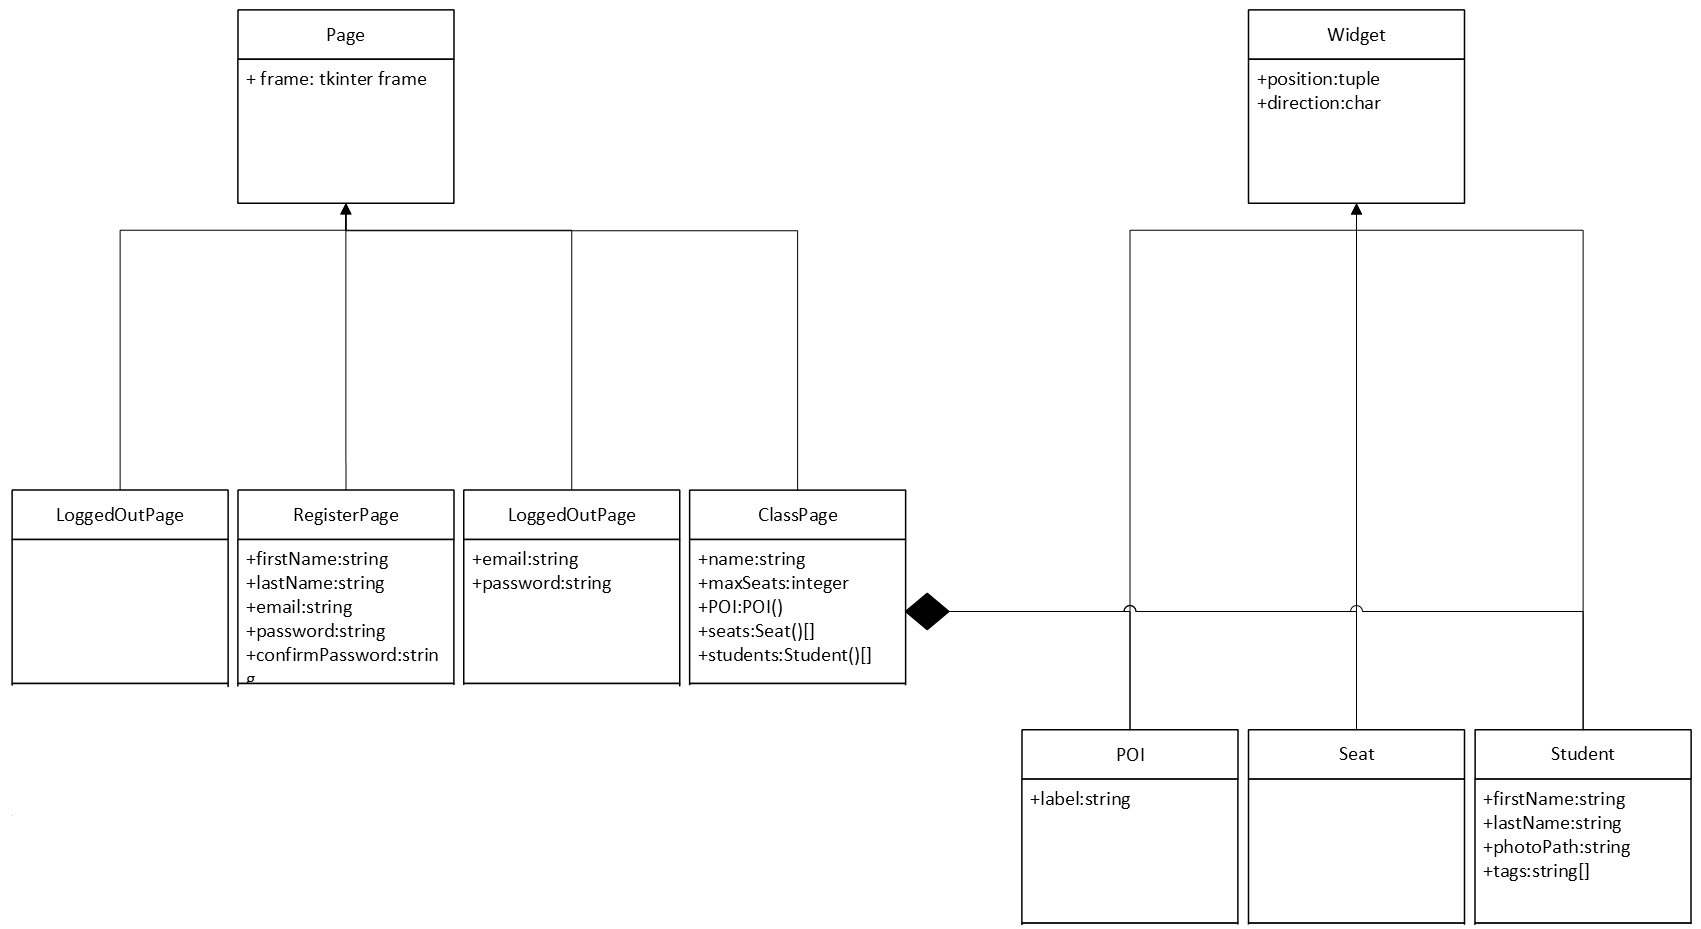
\includegraphics[width=1\linewidth]{ClassAnalysis.png}
    \caption{Class diagram showing relationships between classes and their attributes}
\end{figure}

\begin{figure}[h!]
    \centering
    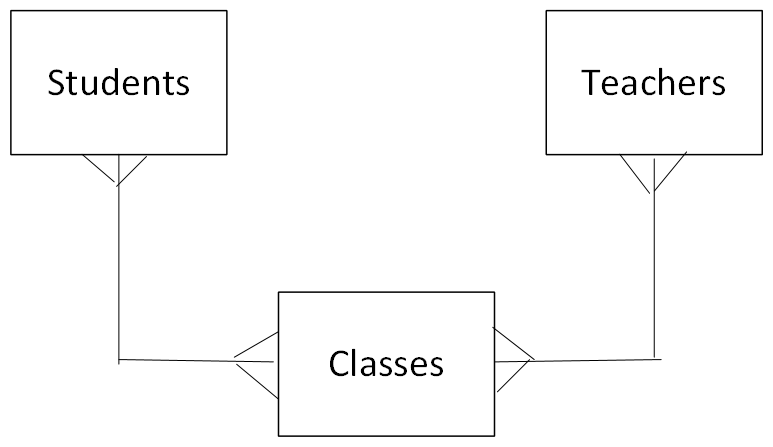
\includegraphics[width=0.5\linewidth]{DatabaseAnalysis.png}
    \caption{Entity relationship diagram between databases that have not yet been normalised}
\end{figure}

\clearpage


\section{Design}


\subsection{Databases}
\hspace{11pt} Teachers(\underline{TeacherID}, FirstName, LastName, Email, Password)

Students(\underline{StudentID}, FirstName, LastName, PhotoPath) 

Classes(\underline{ClassID}, RoomName, MaxSeats)

Seats(\underline{SeatID}, \underline{ClassID}, Position)

Tags(\underline{TagID}, Name, Colour)

StudentClass(\underline{StudentID}, \underline{ClassID}, \underline{SeatID}) 

TeacherClass(\underline{TeacherID}, \underline{ClassID}) 

StudentTags(\underline{StudentID},\underline{TagID})

\subsection{Diagrams}
\begin{figure}[h!]
    \centering
    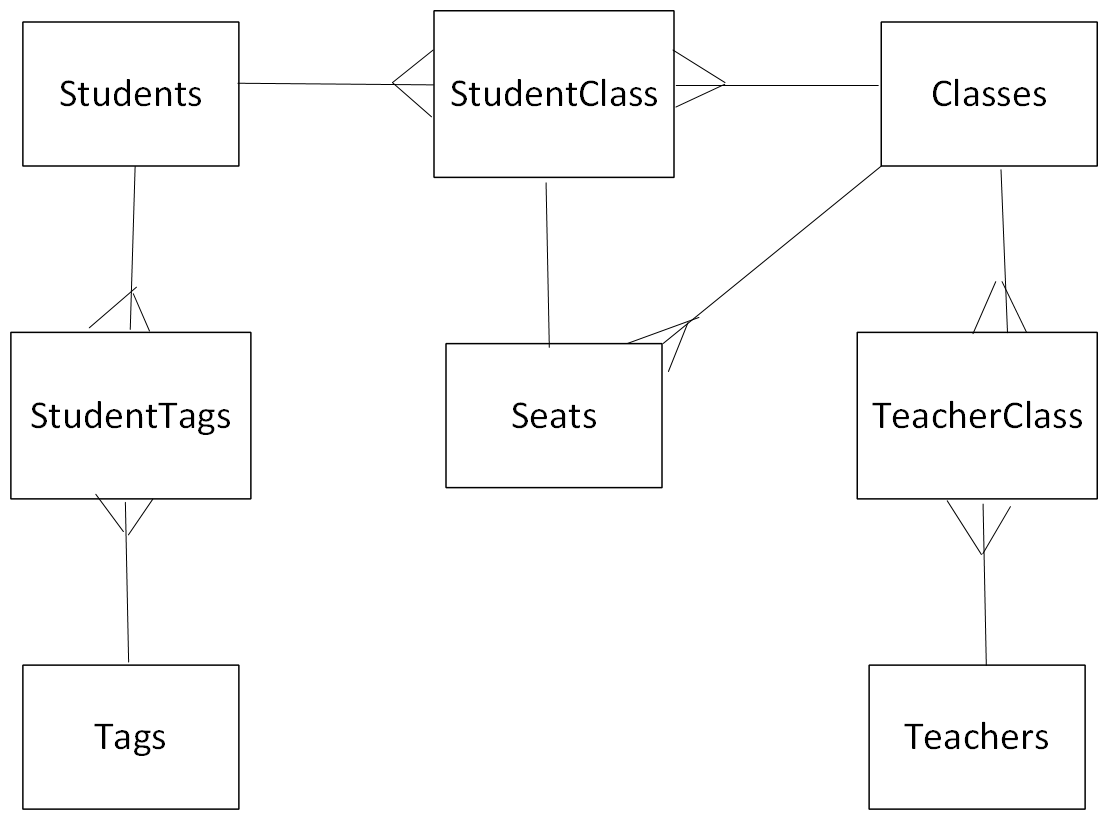
\includegraphics[width=1\linewidth]{DatabaseDesign.png}   
    \caption{Entity relationship diagram between normalised databases}
\end{figure}

\begin{figure}[h!]
    \centering
    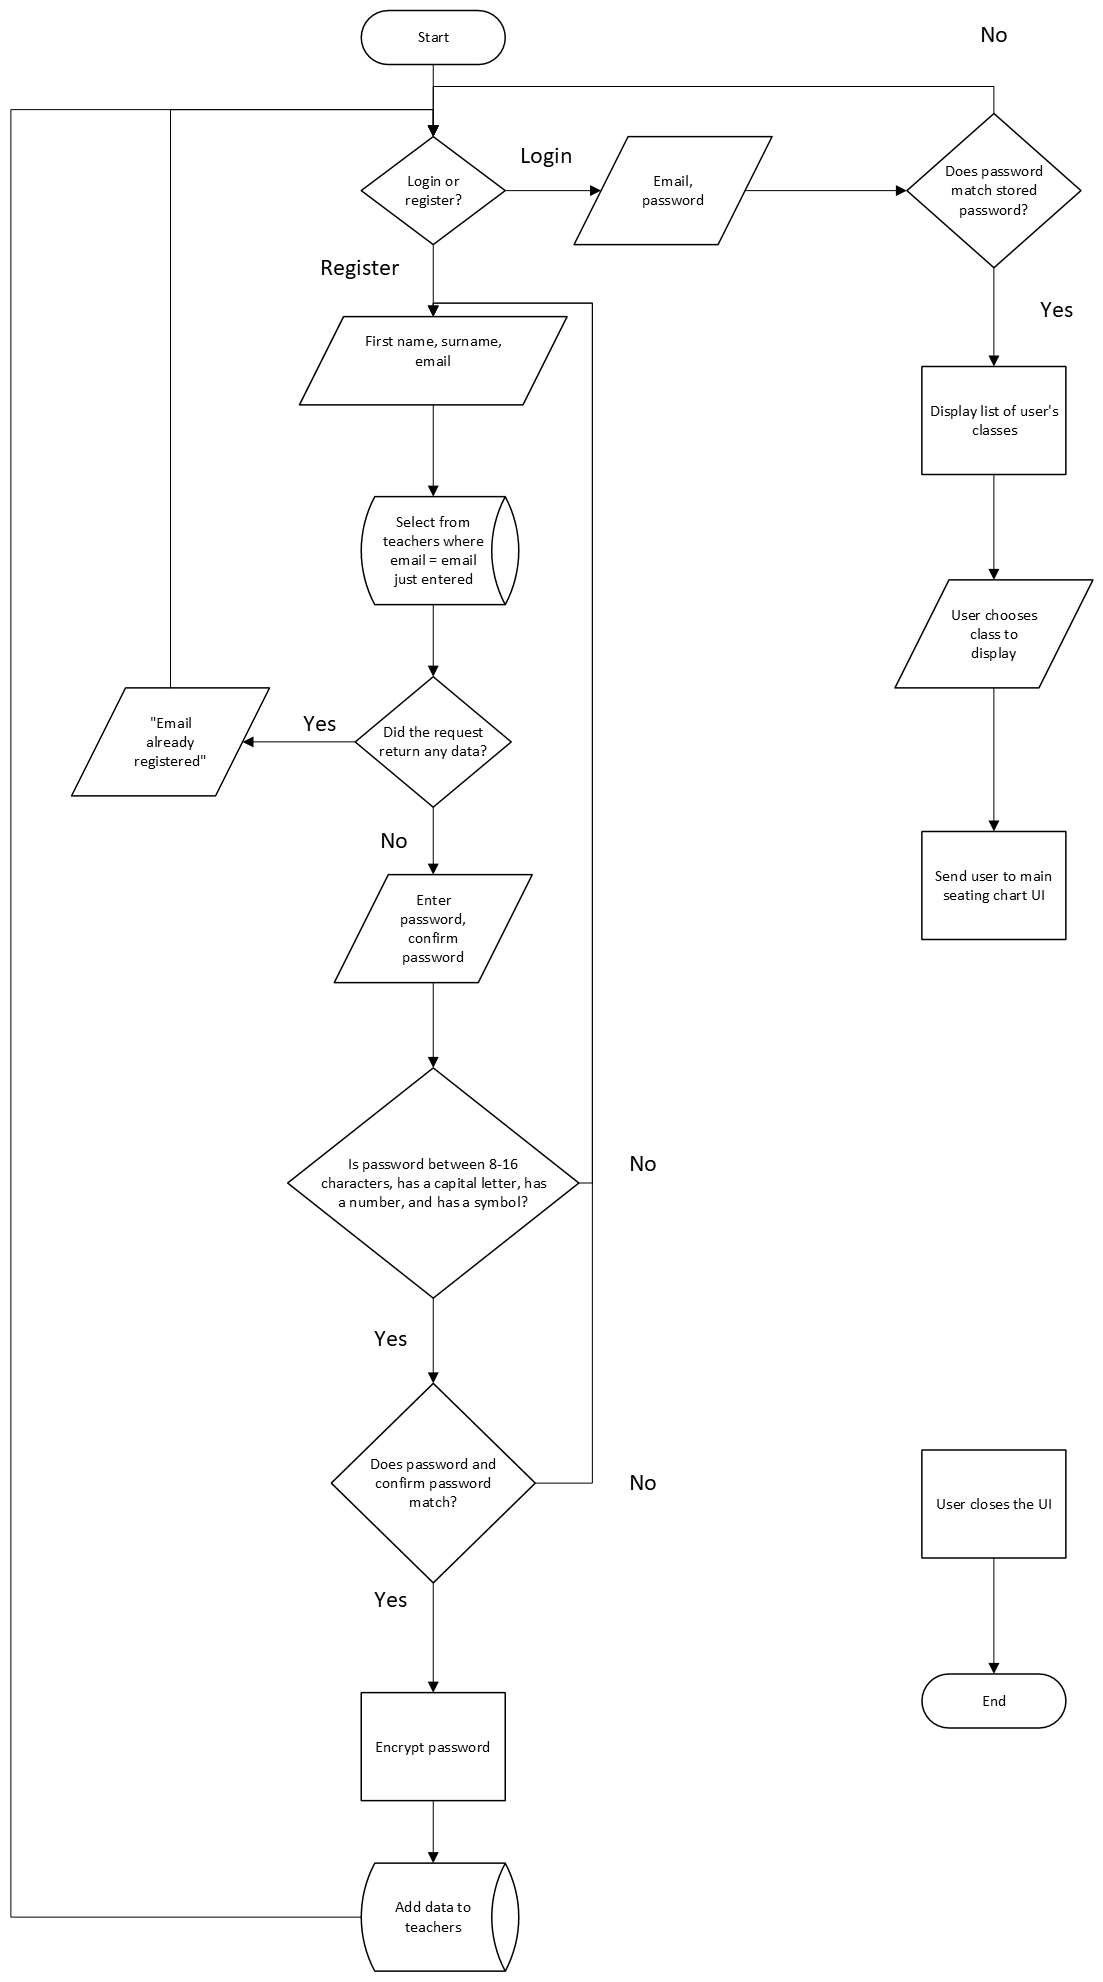
\includegraphics[width=0.84\linewidth]{Register.png}
    \caption{Flowchart for the logging in/registering process}
\end{figure}

\begin{figure}[h!]
    \centering
    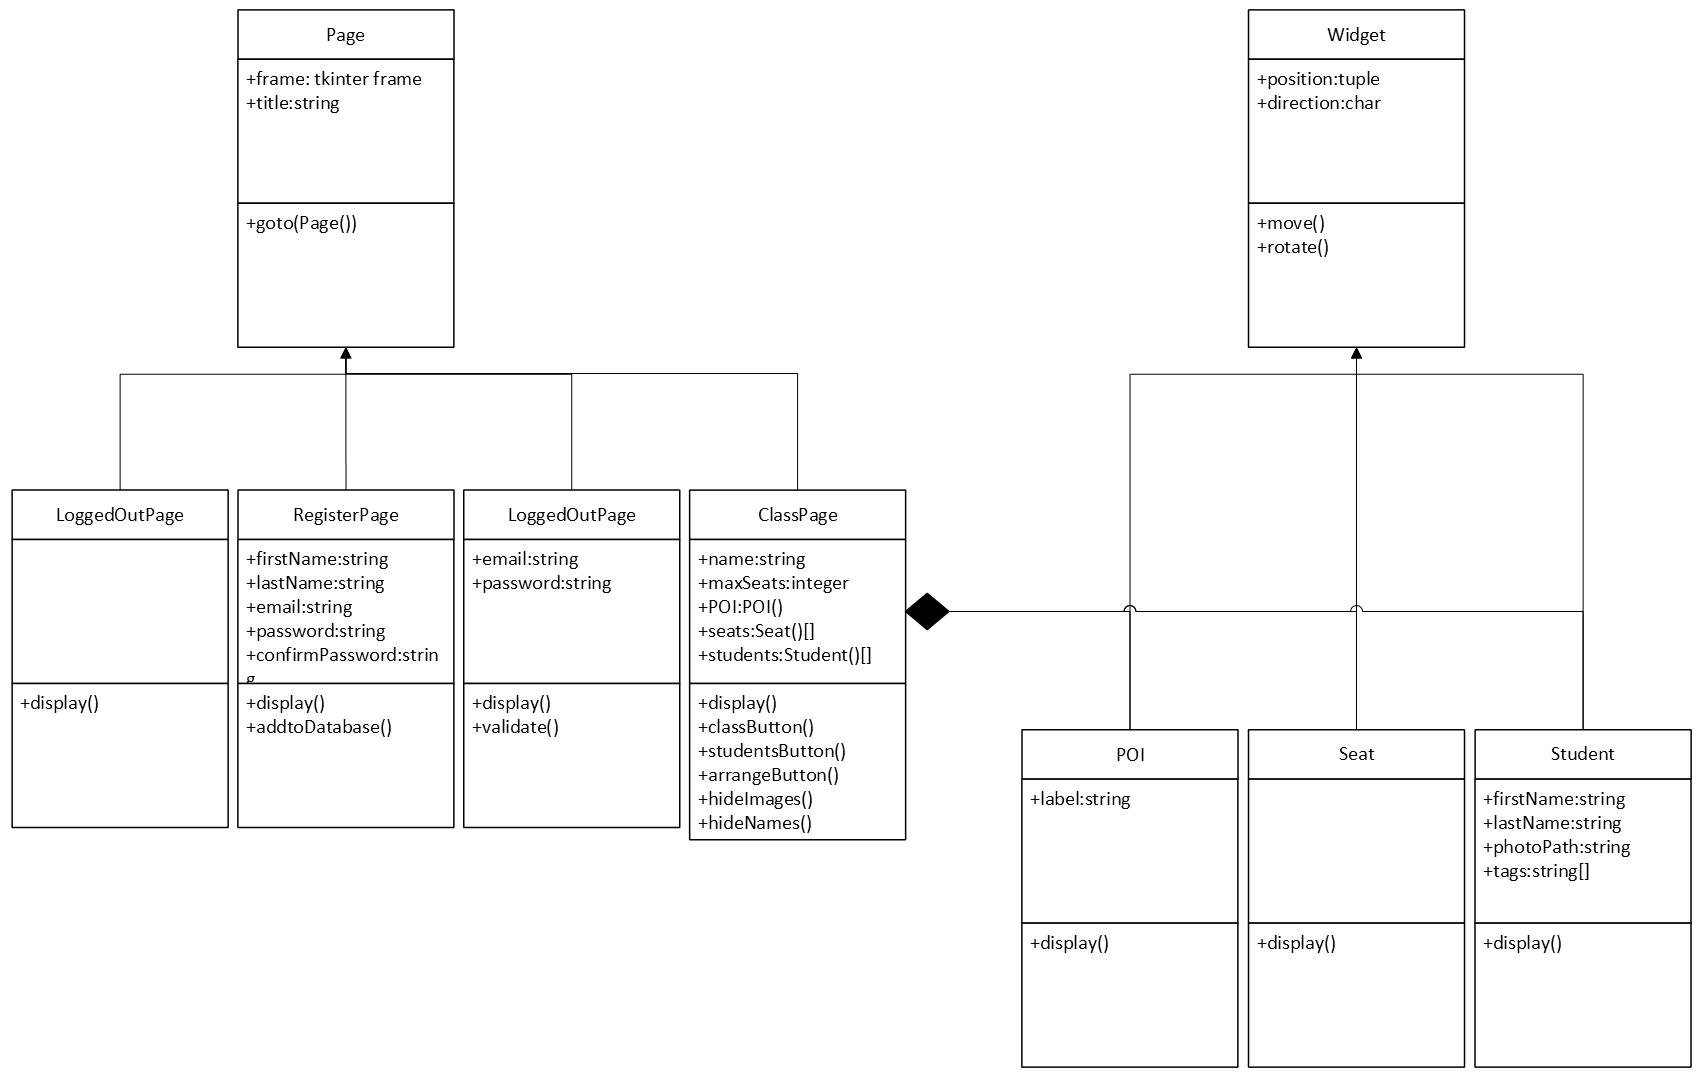
\includegraphics[width=1\linewidth]{ClassDesign.png}
    \caption{Class diagram showing the relationships between classes, attributes, and methods}
\end{figure}


\end{document}
